\clearpage
\begin{flushright}
	\textit{Лекция №12}
	\textit{2016.05.23}
\end{flushright}

Каждый из рассмотренных нами механизмов отложенных дейсвтий выбирается от конкретной ситуации.

 
\begin{lstlisting}[caption=Очереди работ определяются структурой]
<linux/workqueue.h>
struct workqueue_struct
\end{lstlisting}

Очереди работ должны быть созданы до их использования и это можно сделать следующими функциями:
\begin{lstlisting}[caption=Создание очереди работ]
// имеем выделенный поток для каждого ???. Все эти потоки являются лишними.
struct workqueue_struct *create_workqueue(const char *name);

// если одного единственного потока достаточно для все задач, то нужно использовать
struct workqueue_struct *create_singlethread_workqueue(const char *name);
\end{lstlisting}

Чтобы поместить соответствующие дейсвтие в очередь работ, нужно заполнить структуру $work\_struct$ . Это можно сделать во время компиляции макроса:
\begin{lstlisting}
DECLARE_WORK(name, void(*function)(void*), void *data);
\\ name – имя структуры, котороые было объявлено
\\ function – то что будет выполнено в очереди работ.
\end{lstlisting}

Если есть необходимость задать структуру $work\_struct$ динамически, то необходимо использовать следующие 2 макроса:
\begin{lstlisting}
// Делает более тщательную работу по инициализации структуры. Необходимо использовать, если делаем первый раз.
INIT_WORK(struct work_struct *work, void (*function)(void*), void *data);

// Не инициализирует указатели, чтобы связать work_struct с work_queue. Если сущетсвует такая возможность, что представленная структура может исзменяться, то надо использовать PREPARE_WORK
PREPARE_WORK(...);
\end{lstlisting}

\begin{lstlisting}[caption = Функции для отправки работы в очередь работ, label=code_send_work_queue]
// добавляет работку work в определенную очередь.
int queue_work(struct workqueue_strct *queue, struct work_struct *work);

// указывает, что реальная работа не будет выполняться, пока не закнчится установленная задержка.
int queue_delay_work(..., ..., unsigned long delay);
\end{lstlisting}

Функции \ref{code_send_work_queue} возвращают ноль, если работа успешно добавлена в очередь и ненулевой результат, если структура $work\_struct$ уже поставлена в очередь и второй раз она добавлена не будет.

Функция выполняется в контексте потока, которые называется worker thread. Поэтому функция может блокироваться, однако разработчик должен знать как такая блокировка может повлиять на другие задачи в той же самой очереди работ. Функии $work\_queue$ не доступны пользовательские, так как выполняются в потоке ядра. 

Если нужно отменить незавершенный, то 
\begin{lstlisting}
int cancel_delayed_work(struct work_struct *work);
\end{lstlisting}
функция вернет не ноль если вход был отменен до начала выполнения, ядро гарантирует что после вызова она не будет инициирована. Если возвращает ноль, то вход уже начал выполняться каким то процессором, и может еще выполняться и после вызова функции. Чтобы избежать этого и быть увереным что работа не будет выполняться нигде в системе, после того как $cancel\_delayed\_work()$ вернуло 0, нужно выполнить следующий вызов:
\begin{lstlisting}
void flush_workqueue(struct workqueue_struct *queue);
\end{lstlisting}
после возврата из этой функции никакая work, определенная до вызова не будет выполняться ни где в системе. После окончания работы с $work\_queue$ можно удалить её вызовом
\begin{lstlisting}
$void destroy_workqueue(struct workqueue_strct *queue);$
\end{lstlisting}

\subsubsection{Разделяемые очереди}
Драйверы устройств не нуждаются в собственных очередях работ. Если задание только изредка ставится в очередь, то более эффективно использовать разделение уже существующих очередей работ в ядре. Когда разработчик разделяет эти очереди, он должен знать, что разделяет их с другими заданиями. Кроме того, разделение означает, что нельзя монополизировать очередь в течении длительного времени. Кроме того, разработчик должен понимать, что при использовании таких очередей, ваша работа получит процессор через какое то время.

Модуль jiq (just in queue) – экспортирует  2 поля, которые определяют использование разделяемой очереди работ. Используется структура $work\_struct$ которая устанавливается следующим образом:
\begin{lstlisting}
static struct work_struct jiq_work;
/* инициализация */
INIT_WORK(&jiq_work, jiq_print_wq, &jiq_data);
\end{lstlisting}

Для планирования такой работы, которая ставится в разделемую очередь, используется функция:
\begin{lstlisting}
int schedule_work(struct work_struct *work);
\end{lstlisting}

\lstinputlisting[language=c, caption={Функция $jiq\_print\_wq$}, label=code_irq_print_wq]{listing/1.c} 

В функции \ref{code_irq_print_wq} выполняемая работа - это вывод строки, в случае необходимости повторно ставится в очередь. Если пользователь читает задержки устройства, то рабочая функция повторно отправляет себя в отложенный режим с помощью $shedule\_delayed\_work$.

Если нужно отменить $entry\_work$ то используется функци $cancel\_delay\_work$ Однако сброс общей очереди требует вызова специальной функции $flush\_sheduled\_work$. При этом, если не извенстно, кто еще может использовать эту очередь, то реально не известно, сколько рвемени займет возврат из этой функции. Мы должны понимать, что в системе все работы ставятся в очередь, естественно работы представляется потоком. 

\begin{figure}[H]
  \centering
  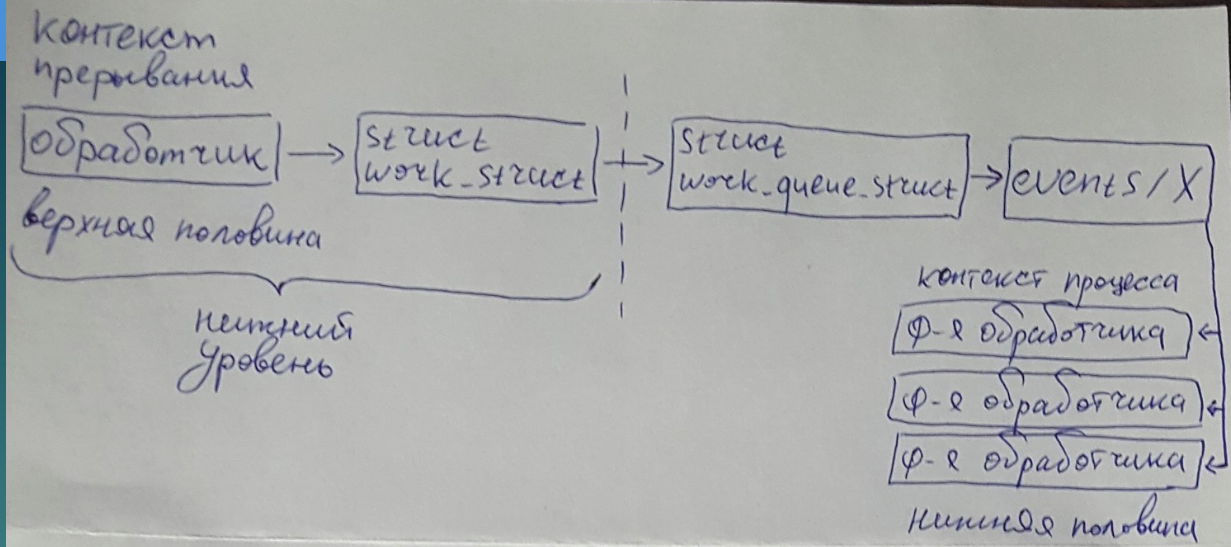
\includegraphics[width=\textwidth]{pic/1.png}
  \caption{pic}
  \label{pic_run_queue_work}
\end{figure}

\ref{pic_run_queue_work} поддерживает эти рассуждения. В основе лежит структура $workqueue\_struct$ куда помещаются данные ???. Потоки ядра events/x выбирают работы из очереди работ и выполняют его. На самом верхнем уровне находятся рабочие потоки, может существовать несколько типов рабочих потоков, для каждого типа рабочих потоков $work\_thread$ существует один рабочий поток на каждый процессор. По умолчанию выполняются только рабочие потоки events которые являются обычными рабочими потоками. Каждый рабочий поток представлен структурой $cpu\_workqueue\_struct$. Стурктура $workqueue\_struct$ представляет ???.

Например можно создать в дополнение к обычному типу потоков events еще один рабочий поток , который назовем $falcon$. На 4-х ядерном компе будет выполняться 4 потока events и следовательно определено 4 экземпляра структуры $cpu\_workqueue\_struct$ и 4 потока $falcon$   для которых также определены структуры  $cpu\_workqueue\_struct$. Для потоков events определен 1 экзампляр структуры $workqueue\_struct$, а для потока $falcon$ дургой экземпляр этой же структуры. 
На самом нижнем уровне находятся отложенные действия, представленные $work\_struct$. Эта структура представлет указатель на обработчик отложенного действия. Отложенное действие отправляется на выполнение определенному потоку. Большинство драйверов использует обычно потоки event.

\chapter{Написание кода драйвера}
В целом, на примере usb драйвера. Затронем вопросы функций, необходимых для регистарции драйвера в системе и т.д.

В системе существует несколько способов классификации драйверов.

По типу:
\begin{enumerate}
	\item симовльных устройств
	\item блочных устройств
	\item драйверы низкого уровня (raw drivers)
\end{enumerate}

В linux по типу:
\begin{enumerate}
	\item драйверы, являющиеся частью кода ядра (встроенные в ядро). Соотсветствующие этим драйверам устройства автоматически обнаруживаются системой и становятся доступными для приложений. Таким образом обеспечивается поддержка устройств для запуска компьютера и монтирования корневой файловой системы. Примеры устройств: видеоконтроллер VGA, контроллеры IDE дисков, материнская крата. последовательные и параллельные порты.
	
	\item драйверы, представленные загружаемыми модулями ядра. Для их установки необходимо выполнять специальные действия, после того как драйвер будет установлен в системе, будет обеспечено управление соответствующего устройства. Если необходимость управления устройством отпало, то такой модуль может быть выгружен. Использование таких загружаемых модулей обеспечивает большую гибкость, так как каждый такой драйвер может быть переконфигурирован без остановки системы. С помощью загружаемых модулей ядра может изменять функциональность внешних устройств. Файлы такие располагаются в $/lib/modules$. $ismod$ выдает спиcок загруженных модулей. $insmod$ – загрузка модуля.

	\item код третьего типа поделен между ядром и специальной утилитой, предназначенной для управления конкретным устройством. Наприме, для принтера ядро отвечает за взаимодейсвтие с параллельным портом, а формировнаие управляющих сигналов для принтера осуществляет демон печати. Другие примеры таких драйверов является драйвер модема и X сервер драйвер видеоадаптера.
\end{enumerate}

\section{Проcтранство имен устройства}

В UNIX существует три различных пространства имен устройства:
\begin{enumerate}
	\item аппаратное, идентифицирует устройство по контроллерам, к которому они подключены, а так же по логическому номеру устройства в контроллере.
	\item  пространство имен устройств ядра. Ядро применяет нумерацию, т.е. старший и младший номера устрйоства.
	\item пространство имен файлов, а именно полные имена файлов. Для пользователя это простое и понятное пространство имен.
\end{enumerate} 

\begin{figure}[H]
  \centering
  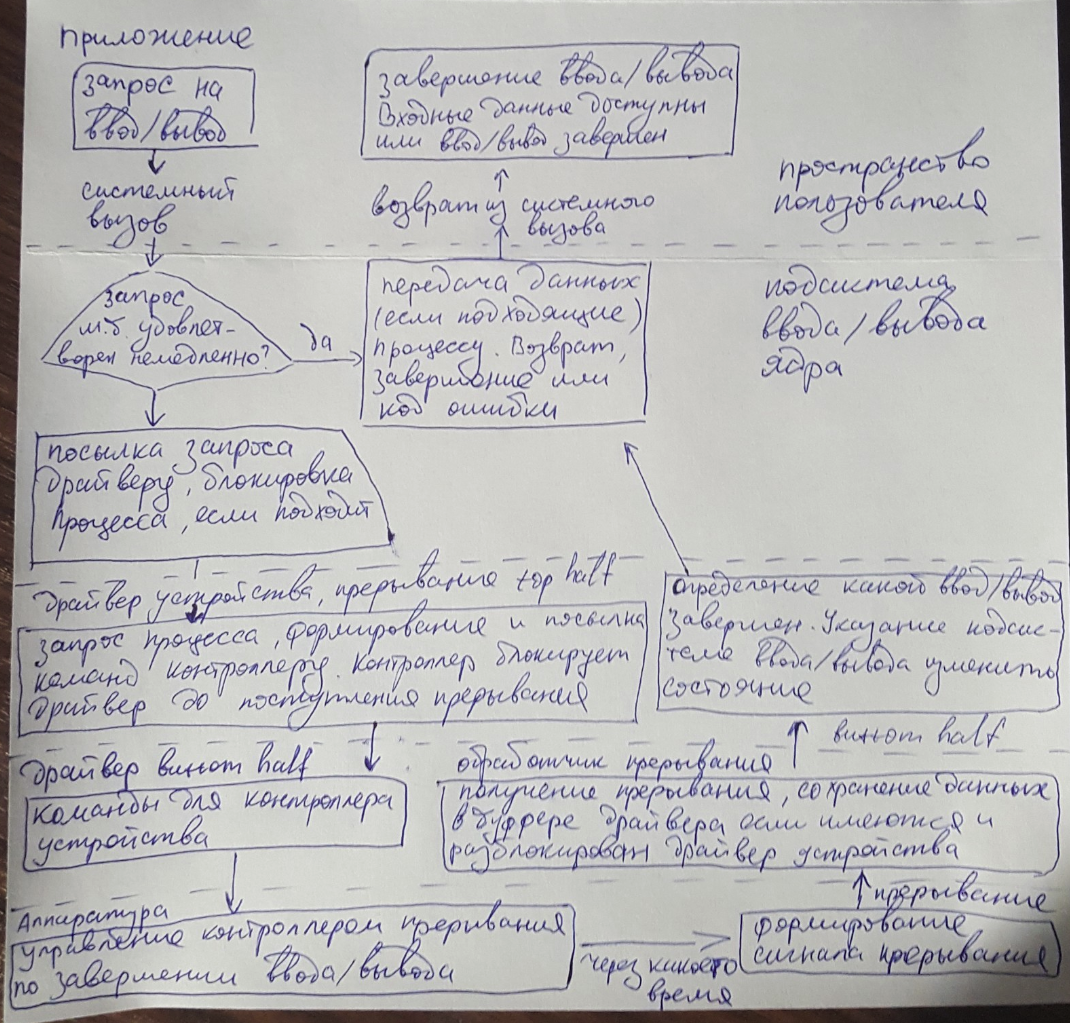
\includegraphics[width=\textwidth]{pic/2.png}
  \caption{pic}
\end{figure}